\documentclass[usenames,dvipsnames, 18pt, compress, aspectratio=169]{beamer}

% can be compiled by xelatex -shell-escape presentation.tex

\usetheme[]{m}

\usepackage[utf8]{inputenc}
\usepackage[russian, english]{babel}
\usepackage{booktabs}
\usepackage[scale=2]{ccicons}
\usepackage{listings}
\usepackage{marvosym}
\usepackage{color}
\usepackage{xcolor}
\usepackage[document]{ragged2e}
\usepackage[export]{adjustbox}
\usepackage{fontawesome}
\usepackage{enumitem}
\usepackage{minted}
\usemintedstyle{tango}
\usepackage[normalem]{ulem}
\usepackage{tikz}
\usetikzlibrary{mindmap}
%\usemintedstyle{monokai}

\usetikzlibrary{shapes,arrows,positioning}
\graphicspath{{images/}}
\newfontfamily{\FA}{FontAwesome}

\definecolor{check}{rgb}{0.1,2,0.3}
\definecolor{fail}{rgb}{2,0.1,0.1}
\definecolor{question}{rgb}{0.9,0.9,0.0}

\def\twitter{{\FA \faTwitter}}
\def\github{{\FA \faGithubSign}}
\def\email{{\FA \faEnvelope}}
\def\check{\textcolor{check}{\FA \faCheck}}
\def\fail{\textcolor{fail}{\FA \faRemove}}
\def\question{\textcolor{question}{\FA \faSearch}}

\renewcommand{\ttdefault}{pcr}
\newfontfamily{\ttfamily}{Fira Code}
\makeatletter
\newcommand\HUGE{\@setfontsize\Huge{32}{41}}
\makeatother

\renewcommand{\ULthickness}{2.0pt}

\definecolor{links}{HTML}{0099FF}
\hypersetup{colorlinks, linkcolor=, urlcolor=links}

\setbeamerfont{section title}{family=\Book, size=\Huge, shape=\normalfont}
\setbeamerfont{frametitle}{family=\Book, size=\large, shape=\normalfont}
\setbeamerfont{title}{family=\Book, size=\HUGE, shape=\normalfont}
\setbeamerfont{subtitle}{size=\LARGE}
\setbeamerfont{author}{family=\ExtraLight, size=\normalsize}
\usebackgroundtemplate{
\includegraphics[width=\paperwidth]{slide_background.png}}

\setbeamertemplate{title page}
{
  \vspace*{3.1cm}
  \begin{columns}[T,onlytextwidth]
  \column{0.3\textwidth}
  \column{0.7\textwidth}
  \begin{minipage}[b][\paperheight]{\textwidth}

    \ifx\inserttitle\@empty\else
    {{% \inserttitle is nonempty
      \raggedright%
      \linespread{1.0}%
      \usebeamerfont{title}%
      \usebeamercolor[fg]{title}%
      \if@noSmallCapitals%
        \inserttitle%
      \else%
        \scshape\MakeLowercase{\inserttitle}%
      \fi%
      \vspace*{0.3em}
    }}
    \fi

    \ifx\insertsubtitle\@empty\else
    {{% \insertsubtitle is nonempty
      \usebeamerfont{subtitle}%
      \usebeamercolor[fg]{subtitle}%
      \insertsubtitle%
      \vspace*{3.5em}%
    }}
    \fi

    \begin{columns}[T,onlytextwidth]
    \column{0.32\textwidth}
      \usebeamerfont{author}%
      \usebeamercolor[fg]{author}%
      \insertauthor%
      \vspace*{0.5em}%
    \column{0.32\textwidth}
      \usebeamerfont{author}%
      \usebeamercolor[fg]{author}%
      Senior Software Engineer
      \vspace*{0.5em}%
    \column{0.32\textwidth}
      \usebeamerfont{author}%
      \usebeamercolor[fg]{author}%
      Zalando
      \vspace*{0.5em}%
    \end{columns}

    \vfill
    \vspace*{2em}
  \end{minipage}
  \end{columns}
}

\setbeamertemplate{section page}
{
  \vspace{2em}
  \centering
  \begin{minipage}{22em}
    \usebeamercolor[fg]{section title}
    \usebeamerfont{section title}
    \insertsectionHEAD\\[-1ex]
  \end{minipage}
  \par
}

\setbeamertemplate{footline}
{
\begin{beamercolorbox}[wd=\textwidth,ht=3ex,dp=3ex,leftskip=0.3cm,rightskip=0.3cm]{structure}
  \usebeamerfont{page number in head/foot}
  \insertframenumber
\end{beamercolorbox}
}

\title{NoSQL внутри SQL}
\subtitle{тактика и стратегия}
\date{\today}
\author{Дмитрий\\ Долгов}
\institute{}

\begin{document}
{
  \usebackgroundtemplate{
\includegraphics[width=\paperwidth]{title_background.png}}%
  \fontsize{17pt}{18}\selectfont
  \maketitle
}

\fontsize{17pt}{19}\selectfont
\section{}

\begin{frame}[fragile]
    \frametitle{}
    \vspace{10pt}
    \begin{itemize}[leftmargin=*, label={\MVRightarrow}]
        \item <+-> Данные бывают разные
        \item <+-> Стандарт SQL/JSON
        \item <+-> Как перестать волноваться\\
                   и начать использовать документы
        \item <+-> Важные факторы,\\
                   влияющие на производительность
        \item <+-> Бенчмарки
        \begin{itemize}[leftmargin=*, label={*}]
            \item <+-> Поиск и чтение документов
            \item <+-> Вставка документов
            \item <+-> Обновление документов
        \end{itemize}
    \end{itemize}
\end{frame}

\begin{frame}[fragile]
    \frametitle{}
    \begin{center}
        \textbf{Данные}
    \end{center}
    \begin{itemize}[leftmargin=*]
        \item <+->
    \end{itemize}

    \vspace{-40pt}

    \begin{columns}[T,onlytextwidth]
    \column{0.5\textwidth}
    \begin{itemize}[leftmargin=*]
        \item <+->
\includegraphics[width=6cm,height=5cm]{relation.png}
    \end{itemize}

    \vspace{20pt}

    \column{0.5\textwidth}
    \begin{itemize}[leftmargin=*]
        \item <+->
\includegraphics[width=6cm,height=5cm]{document.jpg}
    \end{itemize}
    \end{columns}
\end{frame}

\begin{frame}
    \frametitle{}
    \begin{center}
        \textbf{Данные нужно хранить в соответствующем формате:}
        \pause
        \begin{itemize}[label={\MVRightarrow}]
            \item <+-> Отдельные хранилища,\\ единый интерфейс
            \item <+-> Единое хранилище,\\ разные форматы
        \end{itemize}
    \end{center}
\end{frame}

\begin{frame}
    \frametitle{}
    \begin{center}
        \textbf{Отдельные хранилища}
        \pause
        \begin{itemize}[label={\MVRightarrow}]
            \item <+-> Конкретный формат обрабатывается наилучщим образом \check
            \item <+-> Производительность, дублирование \question
            \item <+-> Вопросы интеграции компонентов \fail
        \end{itemize}
    \end{center}
\end{frame}

\begin{frame}
    \frametitle{}
    \begin{center}
        \textbf{Единое хранилище}
        \pause
        \begin{itemize}[label={\MVRightarrow}]
            \item <+-> Не требует интеграции \check
            \item <+-> Производительность, дублирование \question
            \item <+-> Поддержка со стороны БД \question
        \end{itemize}
    \end{center}
\end{frame}
\note{
    если данные разного формата не сравнимы по объему, затраты на интеграцию
    и инфраструктуру могут не окупиться.
}

\usebackgroundtemplate{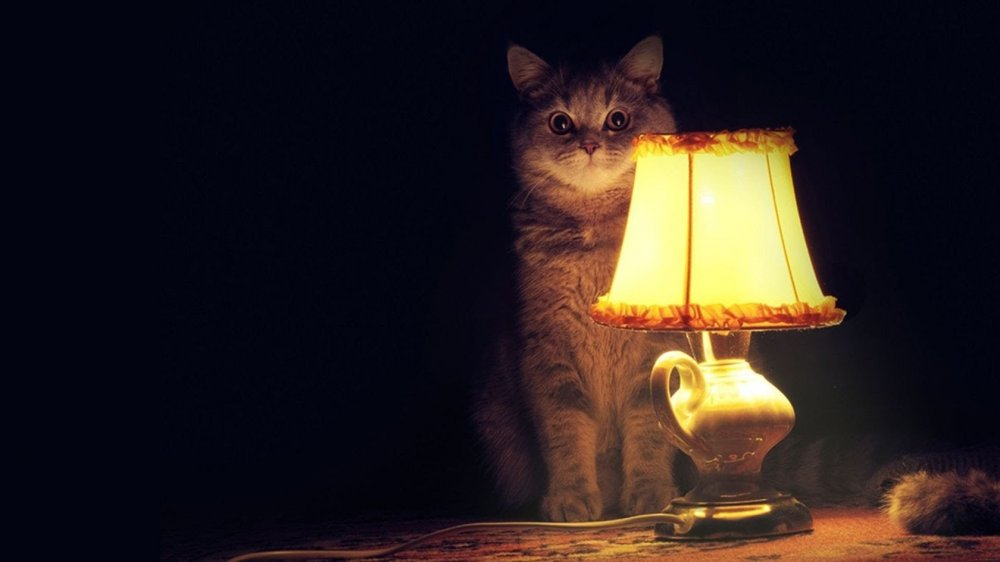
\includegraphics[width=\paperwidth]{cat_stories.jpg}}%
\begin{frame}
    \frametitle{}
\end{frame}

\usebackgroundtemplate{
\includegraphics[width=\paperwidth]{slide_background.png}}
\begin{frame}
    \frametitle{}
    \begin{center}
        \textbf{Кто?}
        \begin{itemize}[label={\MVRightarrow}]
            \item Postgresql (hstore/json/jsonb)
            \item MySQL (json)
            \item Oracle
            \item MSSql
            \item db2
        \end{itemize}
    \end{center}
\end{frame}

\begin{frame}
    \frametitle{}
    \begin{center}
        \textbf{SQL/JSON стандарт}
        \begin{itemize}[label={}]
            \item Опубликован 15.12.2016
            \item Oracle
        \end{itemize}
    \end{center}
\end{frame}

\begin{frame}
    \frametitle{}
    \begin{center}
    \begin{tikzpicture}[
        mindmap, grow cyclic, every node/.style=concept, concept color=orange!40,
        level 1/.append style={level distance=4cm,sibling angle=45},
        level 2/.append style={level distance=2.5cm,sibling angle=45},
        level 3/.append style={level distance=2.5cm,sibling angle=45}]

    \node[scale=0.9] {SQL/JSON}
        child [concept color=blue!30] { node[scale=0.9] {JSON item}
            child [concept color=teal!30] { node[scale=0.9] {scalar}
                child { node[scale=0.9] {text}}
                child { node[scale=0.9] {numeric}}
                child { node[scale=0.9] {boolean}}
                child { node[scale=0.9] {datetime}}
            }
            child { node[scale=0.9] {null}}
            child { node[scale=0.9] {object}}
            child { node[scale=0.9] {array}}
        }
        child [concept color=yellow!30, clockwise from=250] { node[scale=0.9] {JSON sequence} };
    \end{tikzpicture}
    \end{center}
\end{frame}

\begin{frame}
    \frametitle{}
    \begin{center}
    \begin{tikzpicture}[
        mindmap, grow cyclic, every node/.style=concept, concept color=orange!40,
        level 1/.append style={level distance=4cm,sibling angle=45},
        level 2/.append style={level distance=2.5cm,sibling angle=45},
        level 3/.append style={level distance=2.5cm,sibling angle=45}]

    \node[scale=0.9] {Functions}
        child [concept color=teal!40] { node[scale=0.9] {Retrieval}
            child { node[scale=0.9] {Exract value}}
            child { node[scale=0.9] {Exract json}}
            child { node[scale=0.9] {Path existence}}
            child { node[scale=0.9] {Convert to relation}}
            child { node[scale=0.9] {JSON correctness}}
        }
        child [concept color=purple!30, clockwise from=250] { node[scale=0.9] {Construction}
            child { node[scale=0.9] {Create an object}}
            child { node[scale=0.9] {Create an array}}
            child { node[scale=0.9] {Create from relation}}
        };
    \end{tikzpicture}
    \end{center}
\end{frame}

\begin{frame}
    \frametitle{}
    \begin{center}
        \textbf{SQL/JSON стандарт}
        \begin{itemize}[label={\MVRightarrow}]
            \item JSON\_QUERY
            \item JSON item method
            \item JSON filter expression
        \end{itemize}
    \end{center}
\end{frame}

\fontsize{13pt}{14}\selectfont
\begin{frame}
    \frametitle{}
    \vspace{2em}
    \centering
    \begin{minipage}{32em}
        \usebeamercolor[fg]{section title}
        \usebeamerfont{section title}
        Легкий способ начать \sout{бегать по утрам} использовать документы в реляционной базе
    \end{minipage}
\end{frame}
\fontsize{17pt}{18}\selectfont

\usebackgroundtemplate{
\includegraphics[width=\paperwidth]{feature.jpg}}%
\begin{frame}
    \frametitle{}
\end{frame}

\usebackgroundtemplate{
\includegraphics[width=\paperwidth]{slide_background.png}}
\begin{frame}
    \frametitle{}
    \begin{center}
    \inputminted[
        fontsize=\Large,
    ]{sql}{sql/json_build.sql}
    \end{center}
\end{frame}

\begin{frame}
    \frametitle{}
    \begin{center}
    \inputminted[
        fontsize=\Large,
    ]{sql}{sql/json_agg.sql}
    \end{center}
\end{frame}

\begin{frame}
    \frametitle{}
    \begin{center}
    \inputminted[
        fontsize=\Large,
    ]{sql}{sql/load.sql}
    \end{center}
\end{frame}

\begin{frame}
    \frametitle{}
    \begin{center}
        \begin{itemize}[label={\MVRightarrow}]
            \item Загрузка дампа из внешних источников
            \item Некорректные данные с валидной структурой -- json5
            \item Битые данные -- ручное исправление, линтеры
        \end{itemize}
    \end{center}
\end{frame}

\fontsize{13pt}{14}\selectfont
\section{Производительность}
\fontsize{17pt}{18}\selectfont

\begin{frame}
    \frametitle{}
    \begin{center}
        \textbf{Факторы}
        \pause
        \begin{itemize}[label={\MVRightarrow}]
            \item <+-> Структура данных на диске
            \item <+-> Сериализация данных
            \item <+-> Поддержка индексов
        \end{itemize}
    \end{center}
\end{frame}
\note{
    оптимизация по размеру и пробеганию
}

\begin{frame}
    \frametitle{}
    \begin{center}
    \textbf{Bson}
    \begin{figure}
        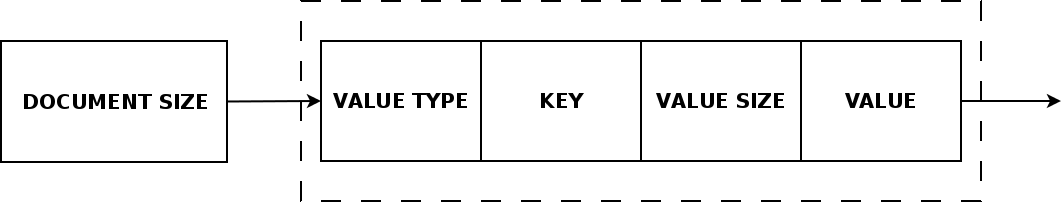
\includegraphics[width=1.0\textwidth,center]{bson.png}
    \end{figure}
    \end{center}
\end{frame}

\begin{frame}
    \frametitle{}
    \begin{center}
    \inputminted[
        fontsize=\Large,
    ]{python}{sql/bson.py}

    \begin{figure}
        
\includegraphics[width=1.0\textwidth,center]{bson_binary.png}
    \end{figure}

    \end{center}
\end{frame}

\begin{frame}
    \frametitle{}
    \begin{center}
    \textbf{Jsonb}
    \begin{figure}
        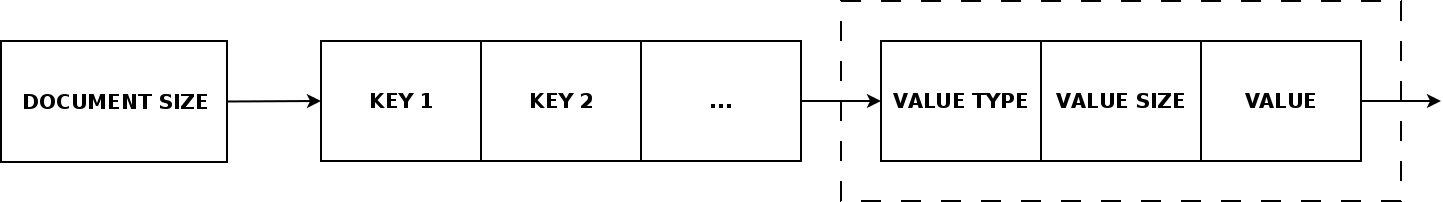
\includegraphics[width=1.0\textwidth,center]{jsonb.png}
    \end{figure}
    \end{center}
\end{frame}

\begin{frame}
    \frametitle{}
    \begin{center}
    \inputminted[
        fontsize=\Large,
    ]{python}{sql/jsonb_binary.sql}

    \begin{figure}
        
\includegraphics[width=1.0\textwidth,center]{jsonb_binary.png}
    \end{figure}

    \end{center}
\end{frame}

\begin{frame}
    \frametitle{}
    \begin{center}
    \textbf{MySQL json}
    \begin{figure}
        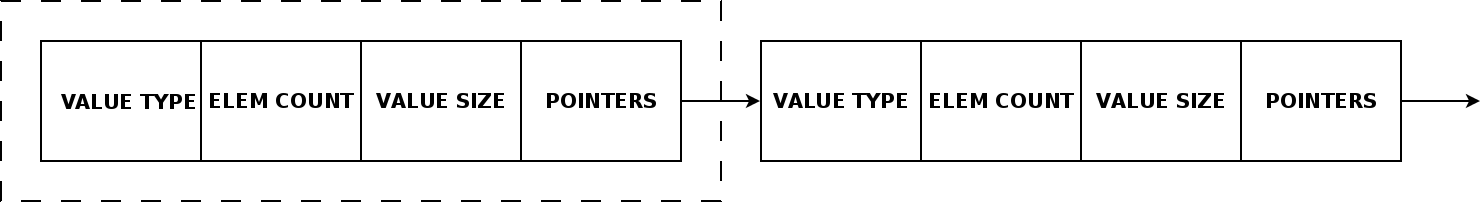
\includegraphics[width=1.0\textwidth,center]{mysql_json.png}
    \end{figure}
    \end{center}
\end{frame}

\begin{frame}
    \frametitle{}
    \textbf{Сериализация данных}
    \begin{center}
        \begin{itemize}[label={\MVRightarrow}]
            \item MongoDB -- дерево Document -> Elements
            \item Postgresql -- JsonbValue со списком элементов
            \item MySQL -- класс Value
        \end{itemize}
    \end{center}
\end{frame}

\begin{frame}
    \frametitle{}
    \textbf{Индексы}
    \begin{center}
        \begin{itemize}[label={\MVRightarrow}]
            \item MongoDB -- индексы для полей
            \item Postgresql -- общий индекс, индексы для полей
            \item MySQL -- виртуальные колонки для индексирования
        \end{itemize}
    \end{center}
\end{frame}

\fontsize{13pt}{14}\selectfont
\section{Тестирование}
\fontsize{17pt}{18}\selectfont

\usebackgroundtemplate{
\includegraphics[width=\paperwidth]{great_performance3.jpg}}%
\begin{frame}
    \frametitle{}
\end{frame}

\usebackgroundtemplate{
\includegraphics[width=\paperwidth]{slide_background.png}}
\begin{frame}
    \frametitle{}
    \begin{center}
        \begin{itemize}[label={}]
            \item PostgreSQL 9.5.4
            \item MySQL 5.7.9
            \item MongoDB 3.2.9
            \item YCSB 0.9
            \item $10^6$ rows and operations
            \item AWS EC2
        \end{itemize}
    \end{center}
\end{frame}

\begin{frame}
    \frametitle{}
    \begin{center}
        \textbf{Воспроизводимость}
        \begin{itemize}[label={}]
            \item \href{https://github.com/erthalion/YCSB}{erthalion/YCSB}
            \item \href{https://github.com/erthalion/ansible-ycsb}{erthalion/ansible-ycsb}
        \end{itemize}
    \end{center}
\end{frame}

\begin{frame}
    \frametitle{}
    \begin{center}
        \textbf{AWS EC2}
        \begin{itemize}[label={}]
            \item m4.xlarge instance
            \item separate instance (database and generator)
            \item 16GB memory, 4 core 2.3GHz
            \item Ubuntu 14.04
            \item Same VPC and placement group
            \item AMI that supports HVM virtualization type
            \item at least 4 rounds of benchmark
        \end{itemize}
    \end{center}
\end{frame}

\begin{frame}
    \frametitle{}
    \begin{center}
        \textbf{Конфигурация}
        \begin{itemize}[label={}]
            \item shared\_buffers
            \item effective\_cache\_size
            \item innodb\_buffer\_pool\_size
            \item write concern level (journaled or transaction\_sync)
        \end{itemize}
    \end{center}
\end{frame}

\begin{frame}
    \frametitle{}
    \begin{center}
        \textbf{Виды документов}
        \begin{itemize}[label={}]
            \item “простой” документ
            \item 10 ключей и значений (100 символов)
            \item 
            \item “большой” документ
            \item 100 ключей и значений (200 символов)
            \item 
            \item “сложный” документ
            \item 100 ключей, 3 уровня вложенности (100 символов)
        \end{itemize}
    \end{center}
\end{frame}

\begin{frame}
    \frametitle{}
    \begin{center}
        \textbf{Простая выборка по ключу с}
        \begin{itemize}[label={}]
            \item "Простой документ"
            \item jsonb\_path\_ops
            \item where data @> '{"key": "value"}'::jsonb
        \end{itemize}
    \end{center}
\end{frame}

\begin{frame}
    \frametitle{}
    \begin{center}
    %\vspace{-10pt}
    \begin{figure}
        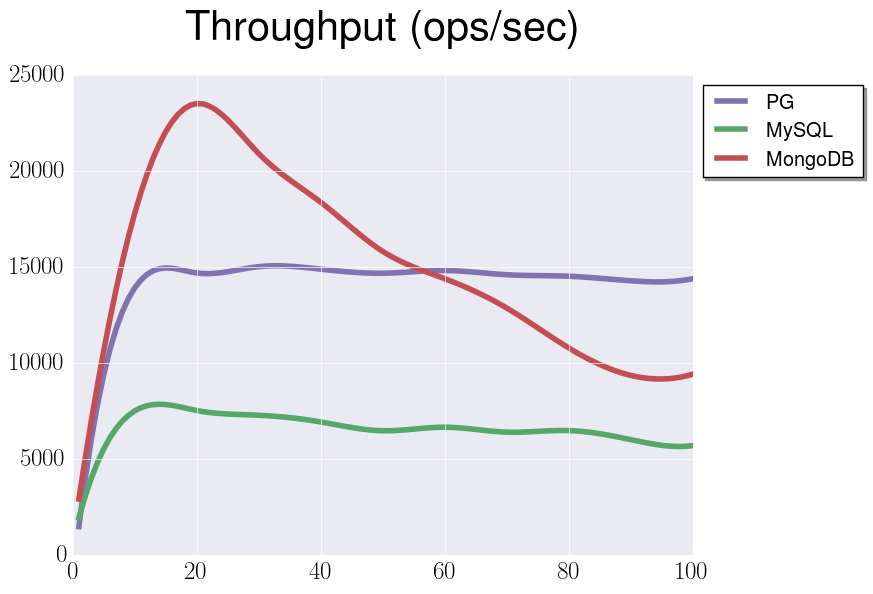
\includegraphics[width=0.75\textwidth,center]{benchmarks/select_jsonb_path_ops_throughput.png}
    \end{figure}
    \end{center}
\end{frame}

\begin{frame}
    \frametitle{}
    \begin{center}
    %\vspace{-10pt}
    \begin{figure}
        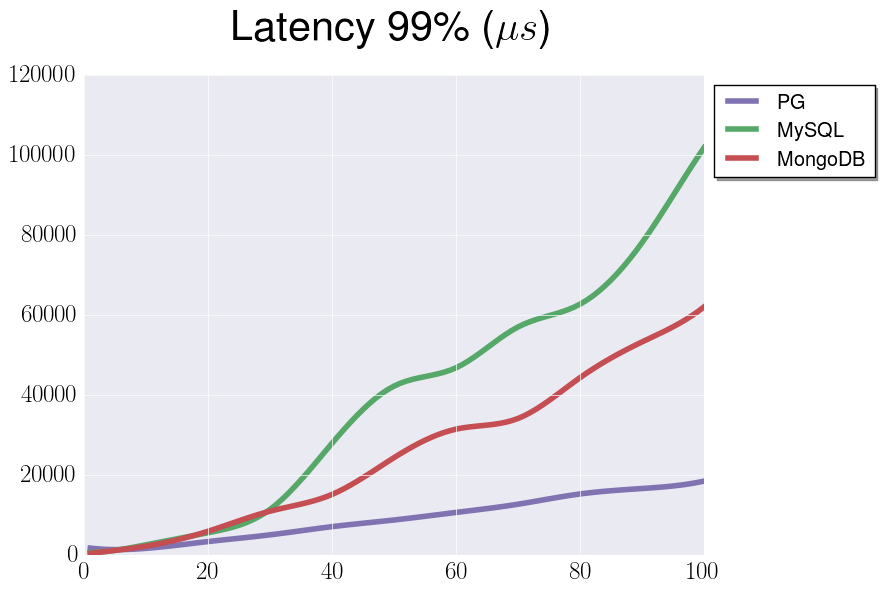
\includegraphics[width=0.75\textwidth,center]{benchmarks/select_jsonb_path_ops_latency_99.png}
    \end{figure}
    \end{center}
\end{frame}

\begin{frame}
    \frametitle{}
    \begin{center}
        \textbf{Простая выборка по ключу}
        \begin{itemize}[label={}]
            \item "Простой документ"
            \item jsonb\_path\_ops
            \item where data @> jsonb\_build\_object('key', 'value')
        \end{itemize}
    \end{center}
\end{frame}

\begin{frame}
    \frametitle{}
    \begin{center}
    %\vspace{-10pt}
    \begin{figure}
        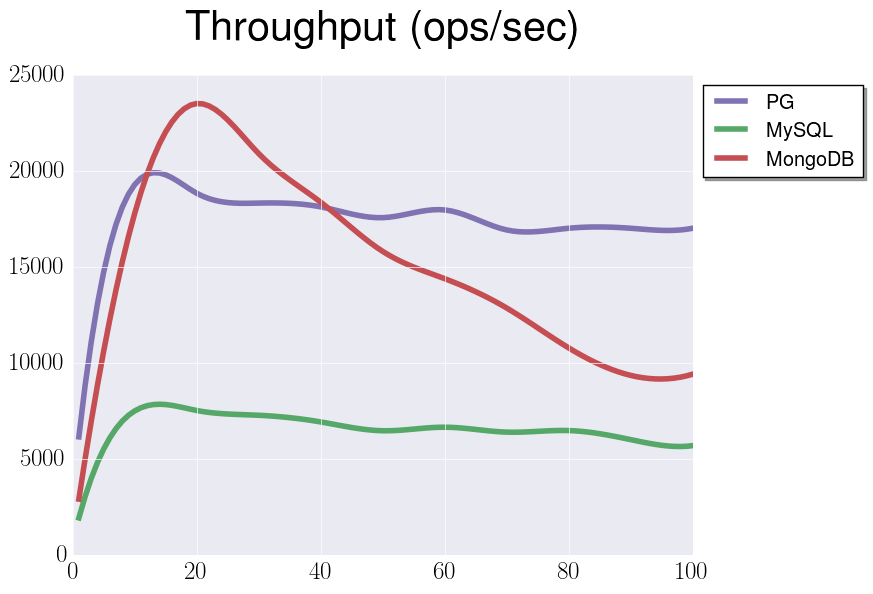
\includegraphics[width=0.75\textwidth,center]{benchmarks/select_jsonb_path_ops_no_parse_throughput.png}
    \end{figure}
    \end{center}
\end{frame}

\begin{frame}
    \frametitle{}
    \begin{center}
        \textbf{Простая выборка по ключу с Btree индексом}
        \begin{itemize}[label={}]
            \item "Простой документ"
            \item btree
        \end{itemize}
    \end{center}
\end{frame}

\begin{frame}
    \frametitle{}
    \begin{center}
    %\vspace{-10pt}
    \begin{figure}
        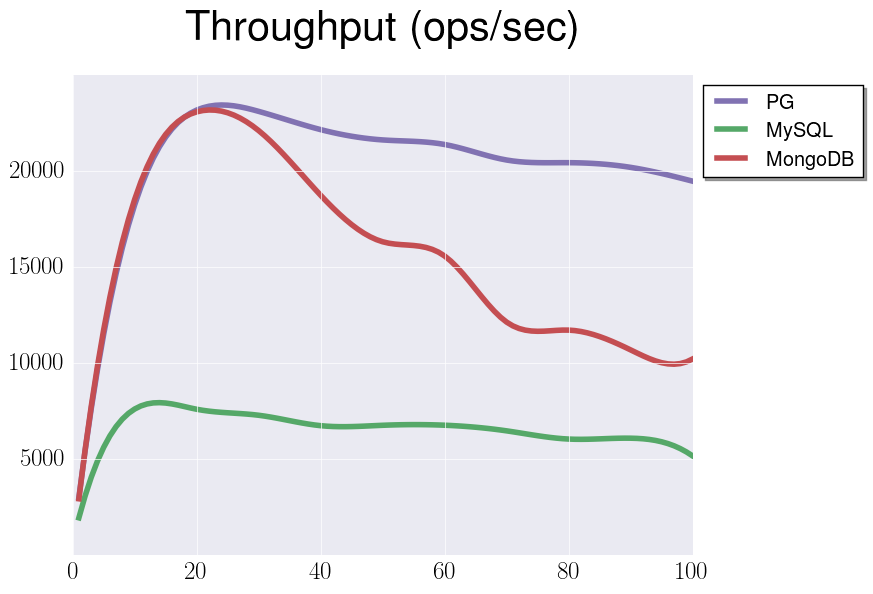
\includegraphics[width=0.75\textwidth,center]{benchmarks/select_btree_throughput.png}
    \end{figure}
    \end{center}
\end{frame}

\begin{frame}
    \frametitle{}
    \begin{center}
    %\vspace{-10pt}
    \begin{figure}
        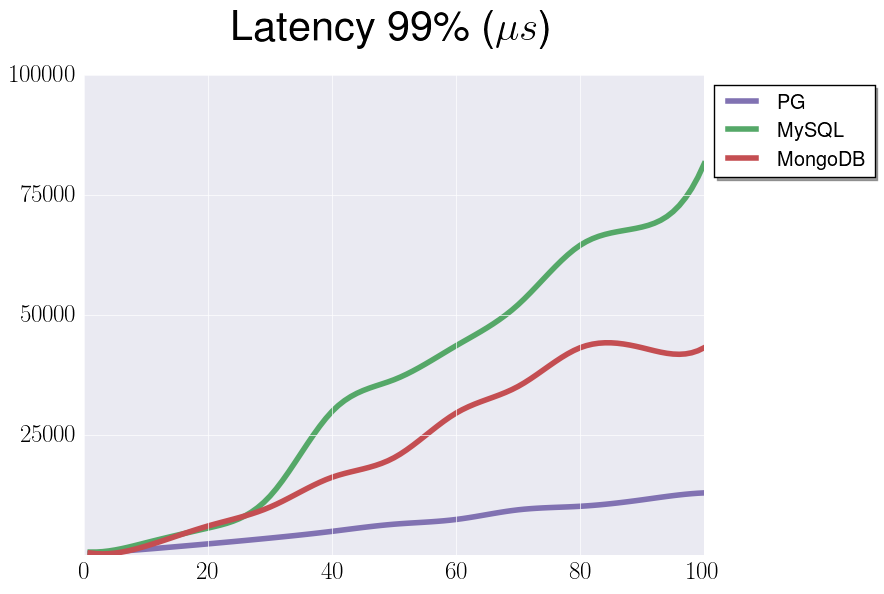
\includegraphics[width=0.75\textwidth,center]{benchmarks/select_btree_latency.png}
    \end{figure}
    \end{center}
\end{frame}

\begin{frame}
    \frametitle{}
    \begin{center}
        \textbf{Простая выборка по ключу с Btree индексом}
        \begin{itemize}[label={}]
            \item "Сложный документ"
            \item btree
        \end{itemize}
    \end{center}
\end{frame}

\begin{frame}
    \frametitle{}
    \begin{center}
    %\vspace{-10pt}
    \begin{figure}
        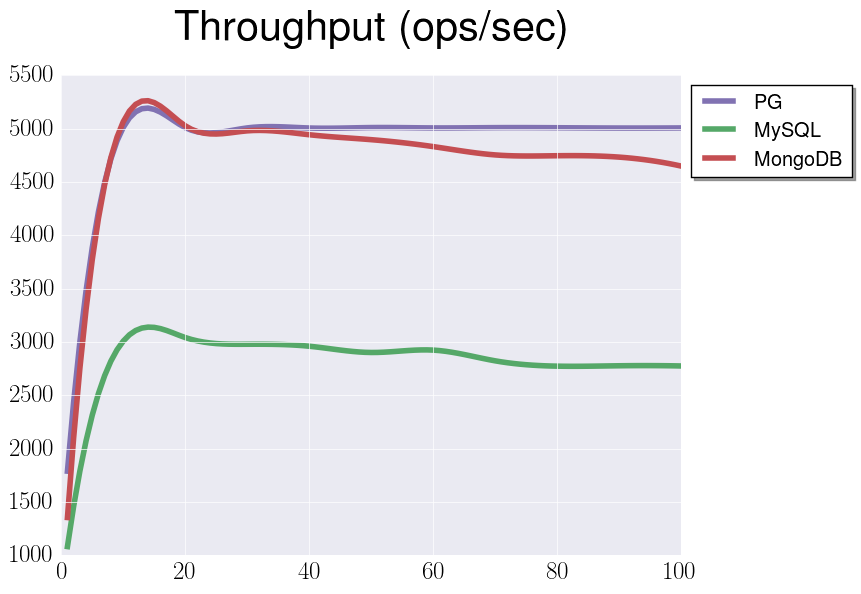
\includegraphics[width=0.75\textwidth,center]{benchmarks/select_complex_btree_throughput.png}
    \end{figure}
    \end{center}
\end{frame}

%\begin{frame}
    %\frametitle{}
    %\begin{center}
    %%\vspace{-10pt}
    %\begin{figure}
        %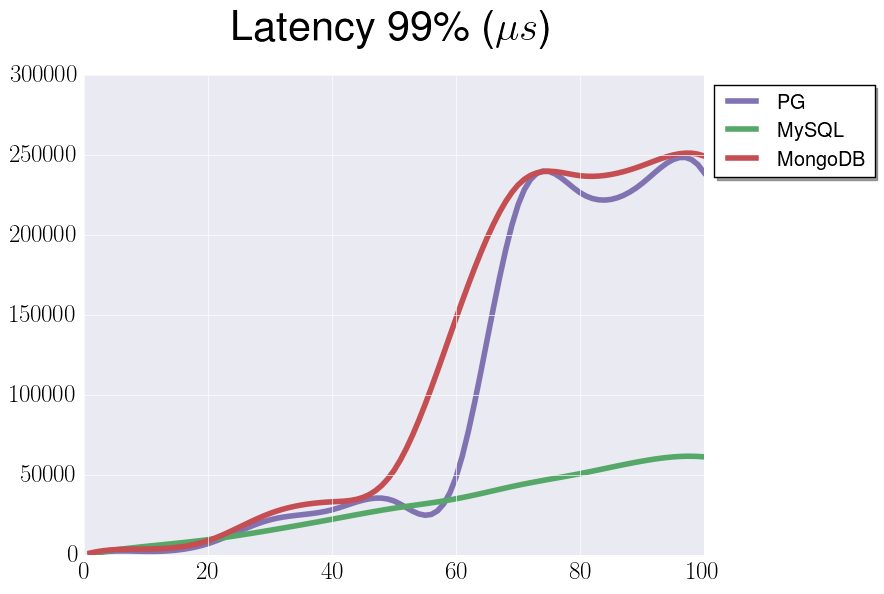
\includegraphics[width=0.75\textwidth,center]{benchmarks/select_complex_btree_latency_99.png}
    %\end{figure}
    %\end{center}
%\end{frame}

\begin{frame}
    \frametitle{}
    \begin{center}
        \textbf{Срез по документу}
        \begin{itemize}[label={}]
            \item "Большой документ"
            \item Из документа выбирается одно поле
        \end{itemize}
    \end{center}
\end{frame}

\begin{frame}
    \frametitle{}
    \begin{center}
    %\vspace{-10pt}
    \begin{figure}
        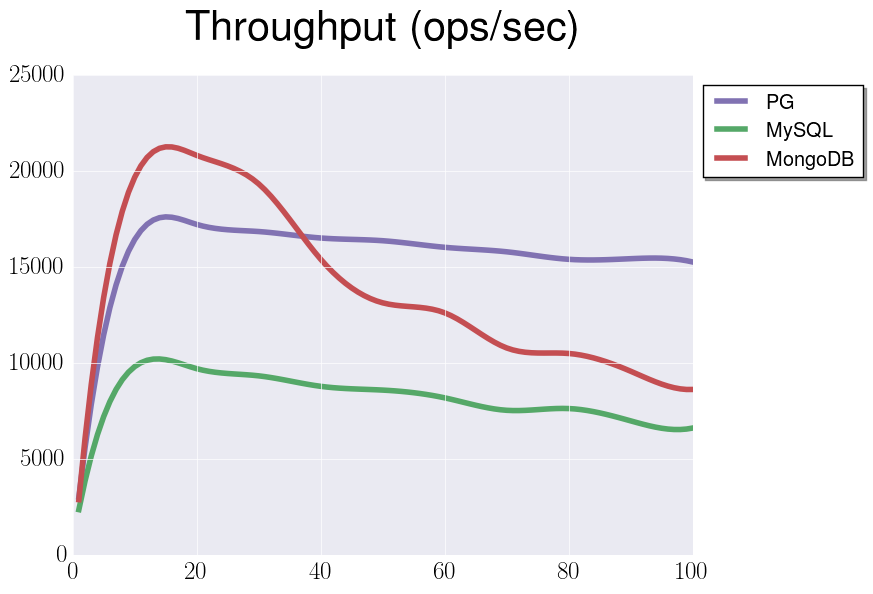
\includegraphics[width=0.75\textwidth,center]{benchmarks/select_slice_1_btree_throughput.png}
    \end{figure}
    \end{center}
\end{frame}

\begin{frame}
    \frametitle{}
    \begin{center}
        \textbf{Срез по документу}
        \begin{itemize}[label={}]
            \item "Большой документ"
            \item Из документа выбирается 10 полей
        \end{itemize}
    \end{center}
\end{frame}

\begin{frame}
    \frametitle{}
    \begin{center}
    %\vspace{-10pt}
    \begin{figure}
        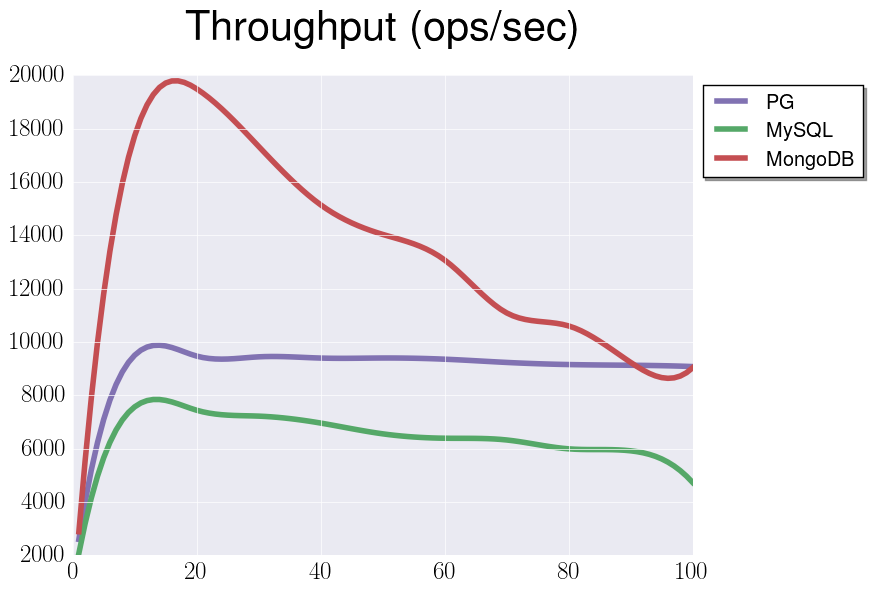
\includegraphics[width=0.75\textwidth,center]{benchmarks/select_slice_10_btree_throughput.png}
    \end{figure}
    \end{center}
\end{frame}

\usebackgroundtemplate{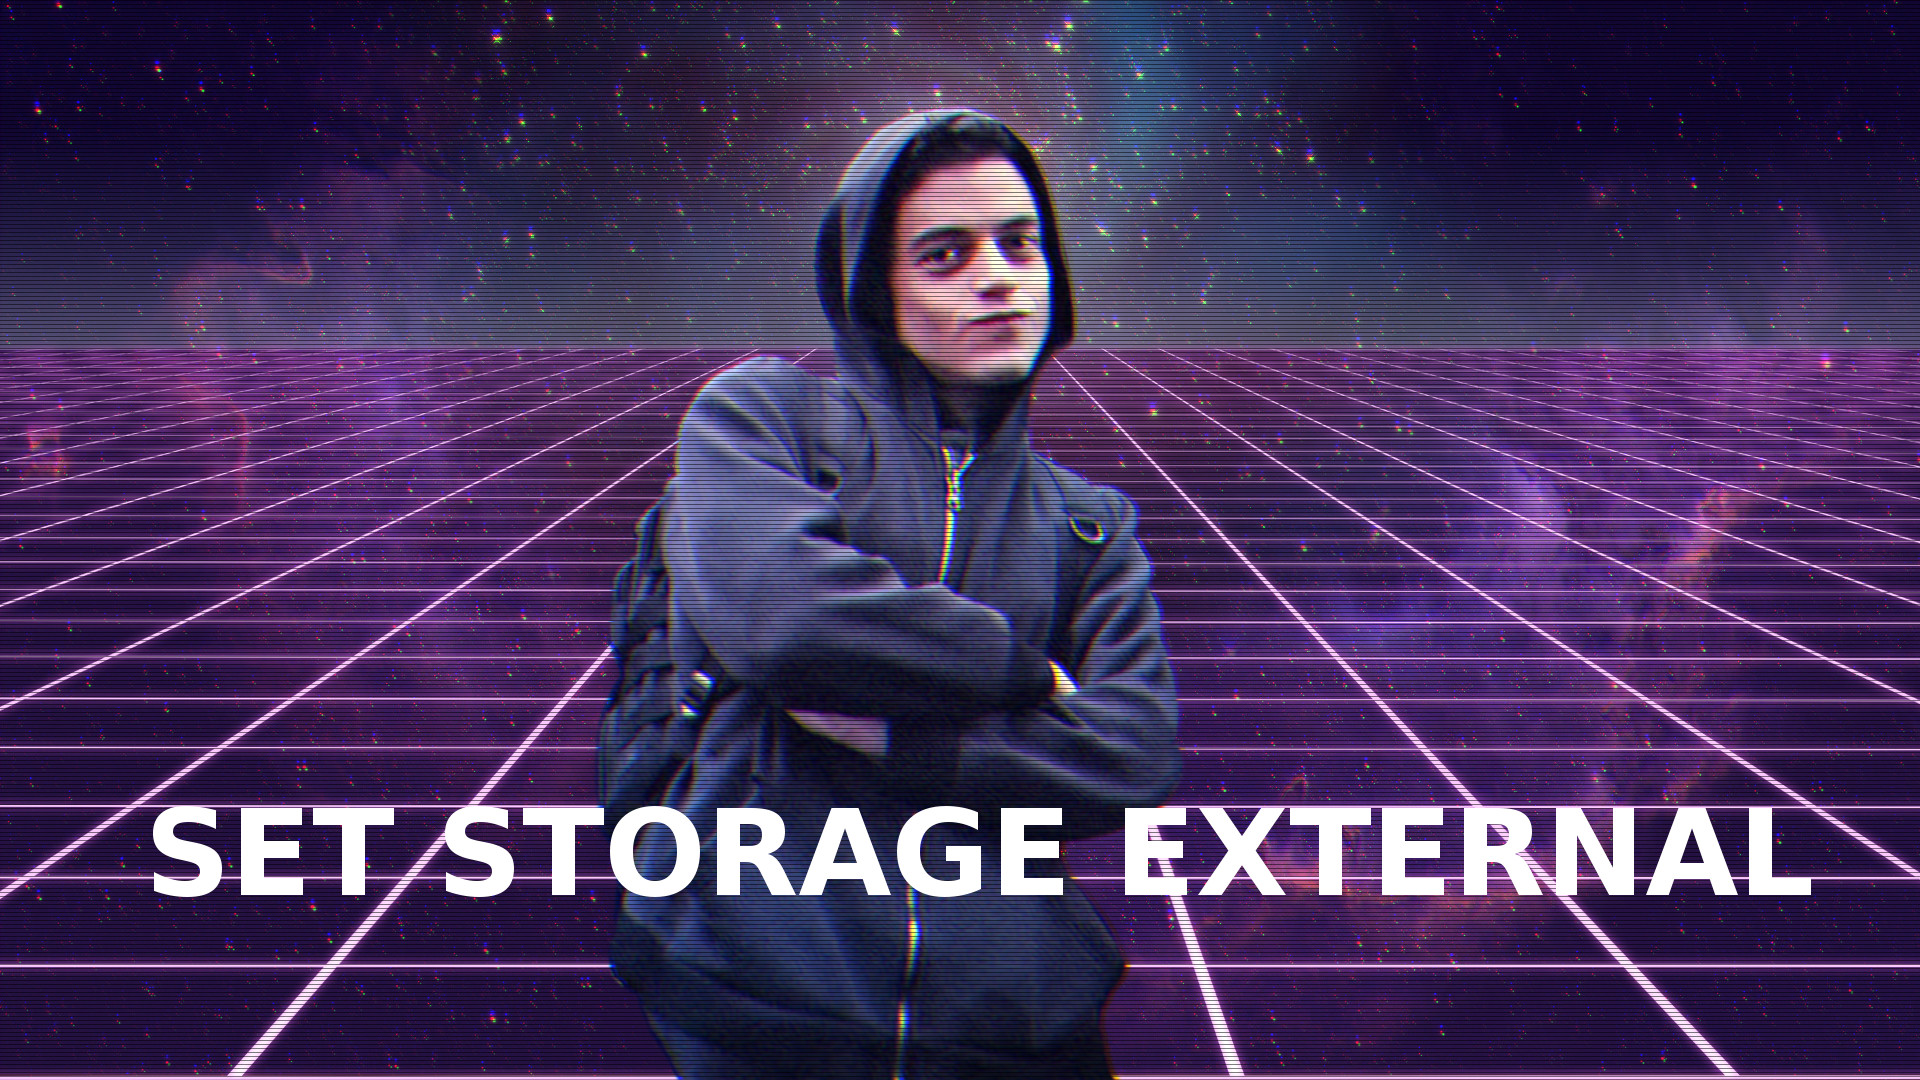
\includegraphics[width=\paperwidth]{hack.jpg}}%
\begin{frame}
    \frametitle{}
\end{frame}

\usebackgroundtemplate{
\includegraphics[width=\paperwidth]{slide_background.png}}
\begin{frame}
    \frametitle{}
    \begin{center}
        \textbf{Масштабируемость}
        \begin{itemize}[label={}]
            \item "Простой документ"
            \item m4.large
            \item m4.xlarge
            \item m4.2xlarge
        \end{itemize}
    \end{center}
\end{frame}

\begin{frame}
    \frametitle{}
    \begin{center}
    %\vspace{-10pt}
    \begin{figure}
        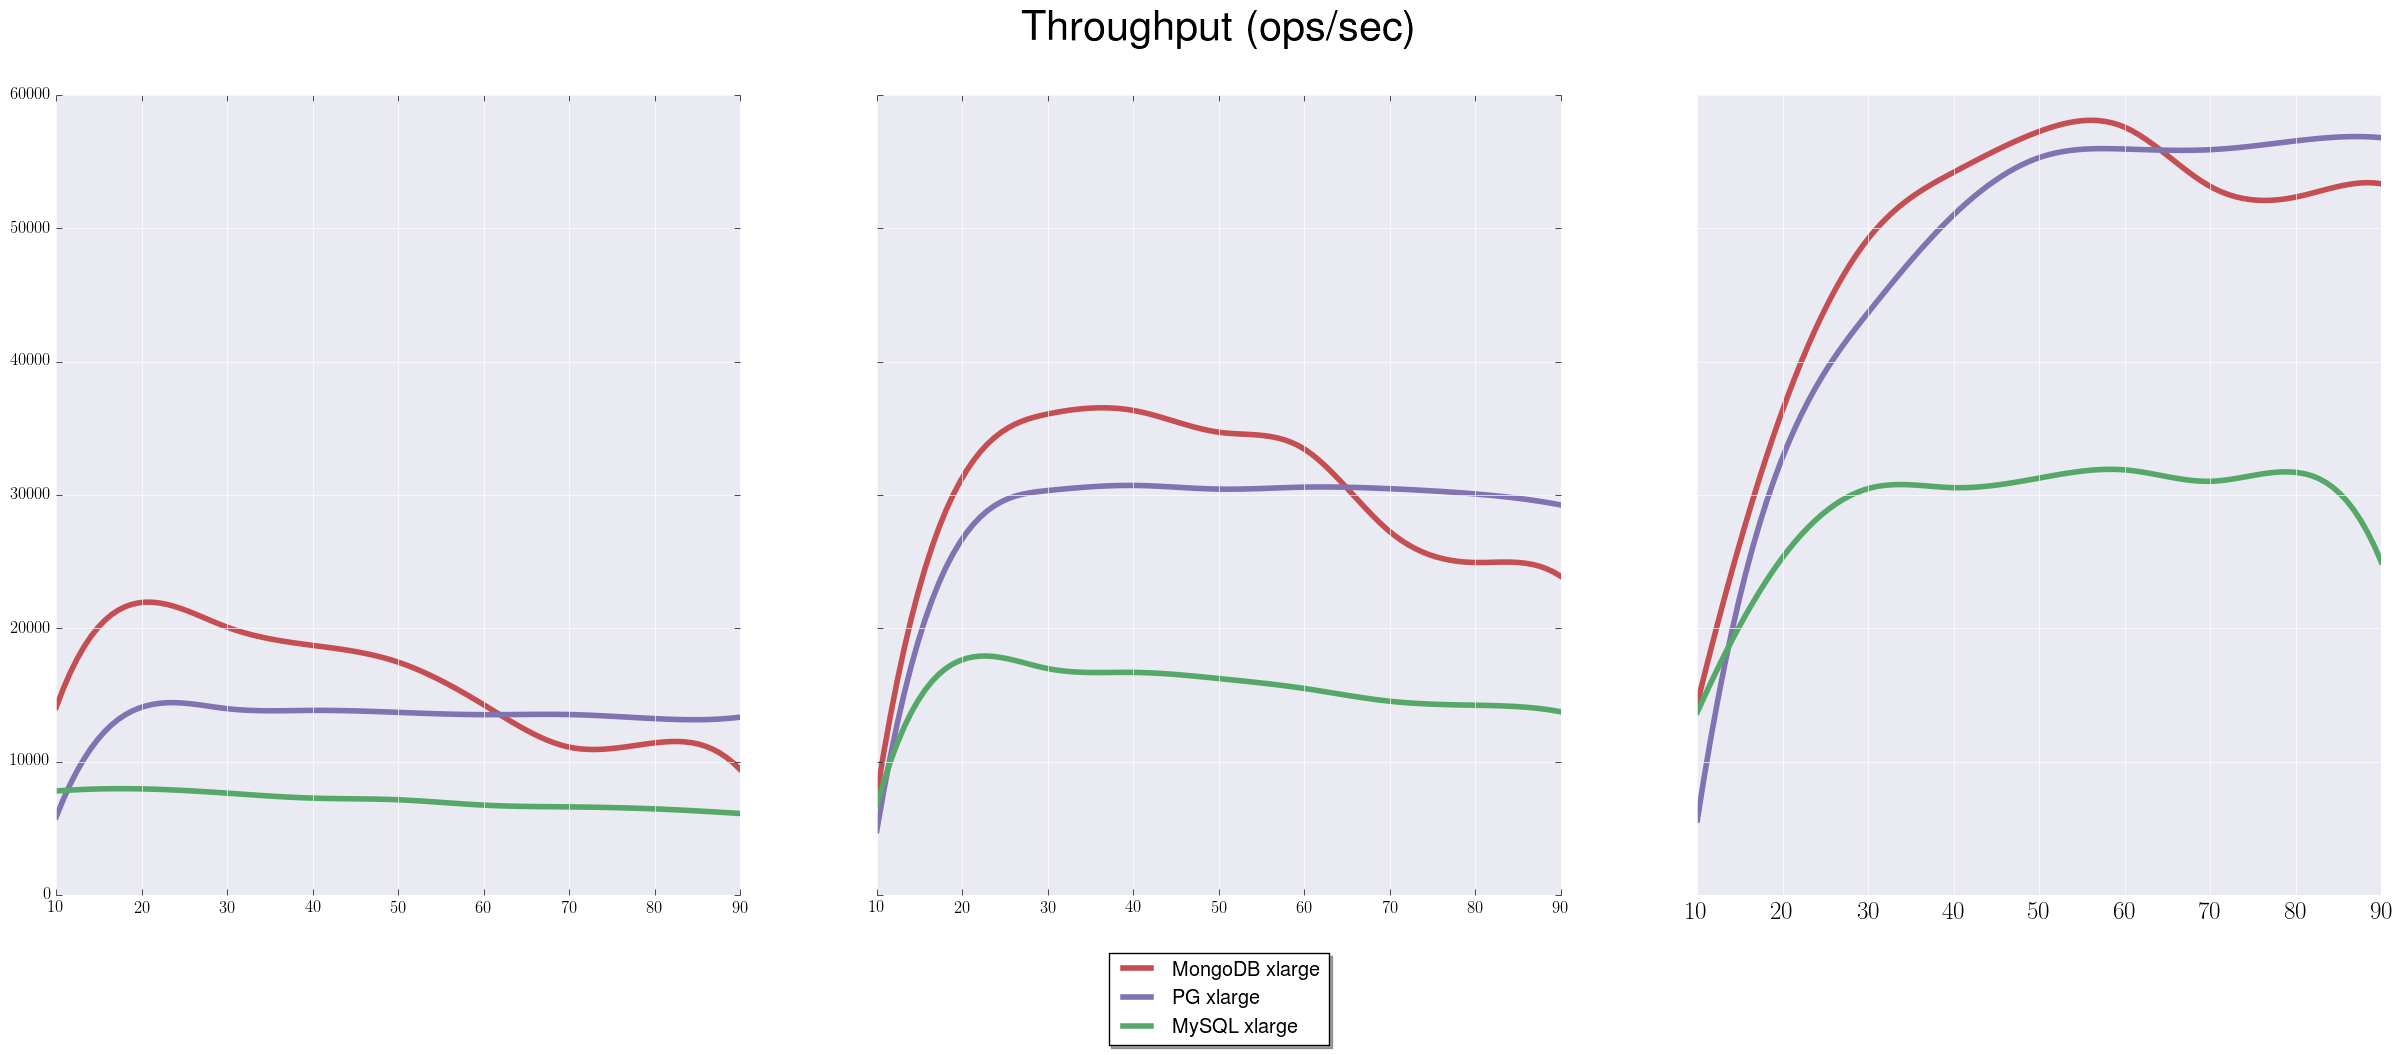
\includegraphics[height=8cm,width=1.1\textwidth,center]{benchmarks/scalability_select_throughput.png}
    \end{figure}
    \end{center}
\end{frame}

%\begin{frame}
    %\frametitle{}
    %\begin{center}
    %\vspace{-10pt}
    %\textbf{Простая выборка по ключу с индексом}
    %\begin{figure}
        %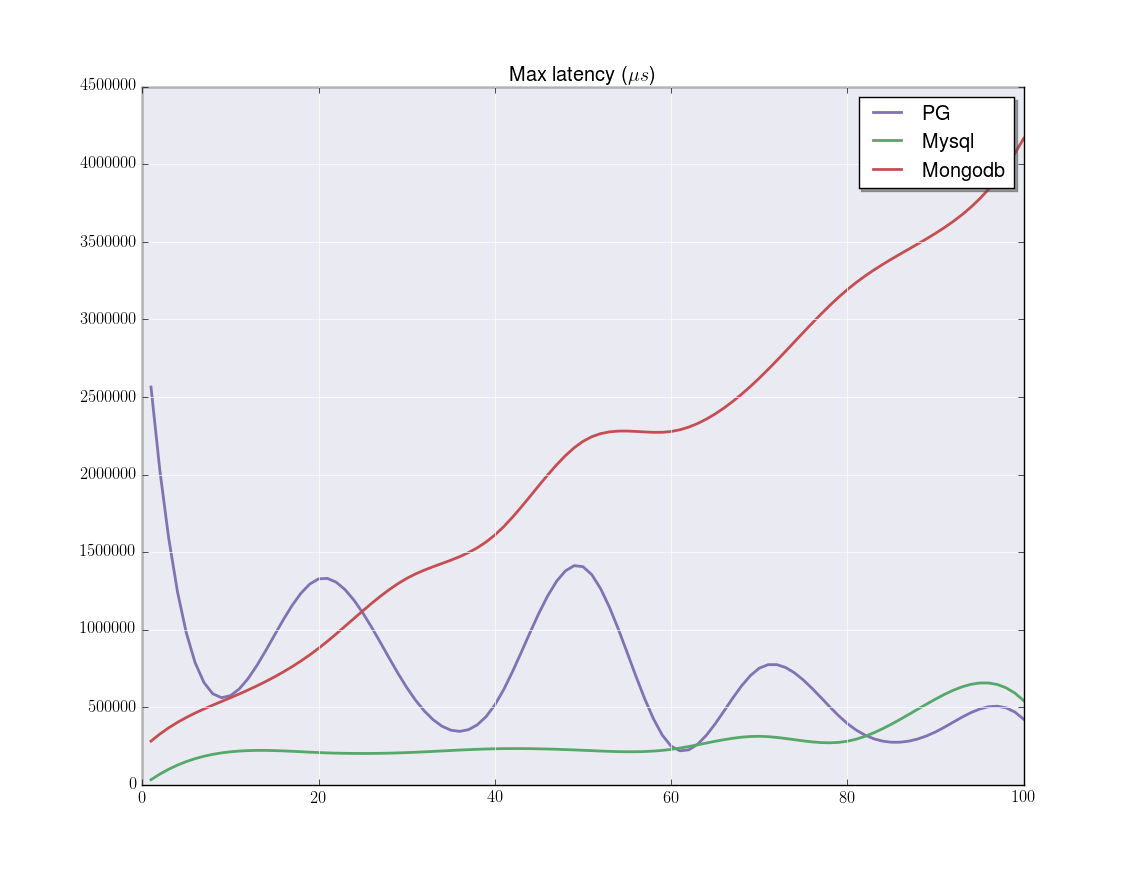
\includegraphics[width=0.7\textwidth,center]{benchmarks/simple_select_max_latency.png}
    %\end{figure}
    %\end{center}
%\end{frame}

%\begin{frame}
    %\frametitle{}
    %\begin{center}
    %%\vspace{-10pt}
    %\begin{figure}
        %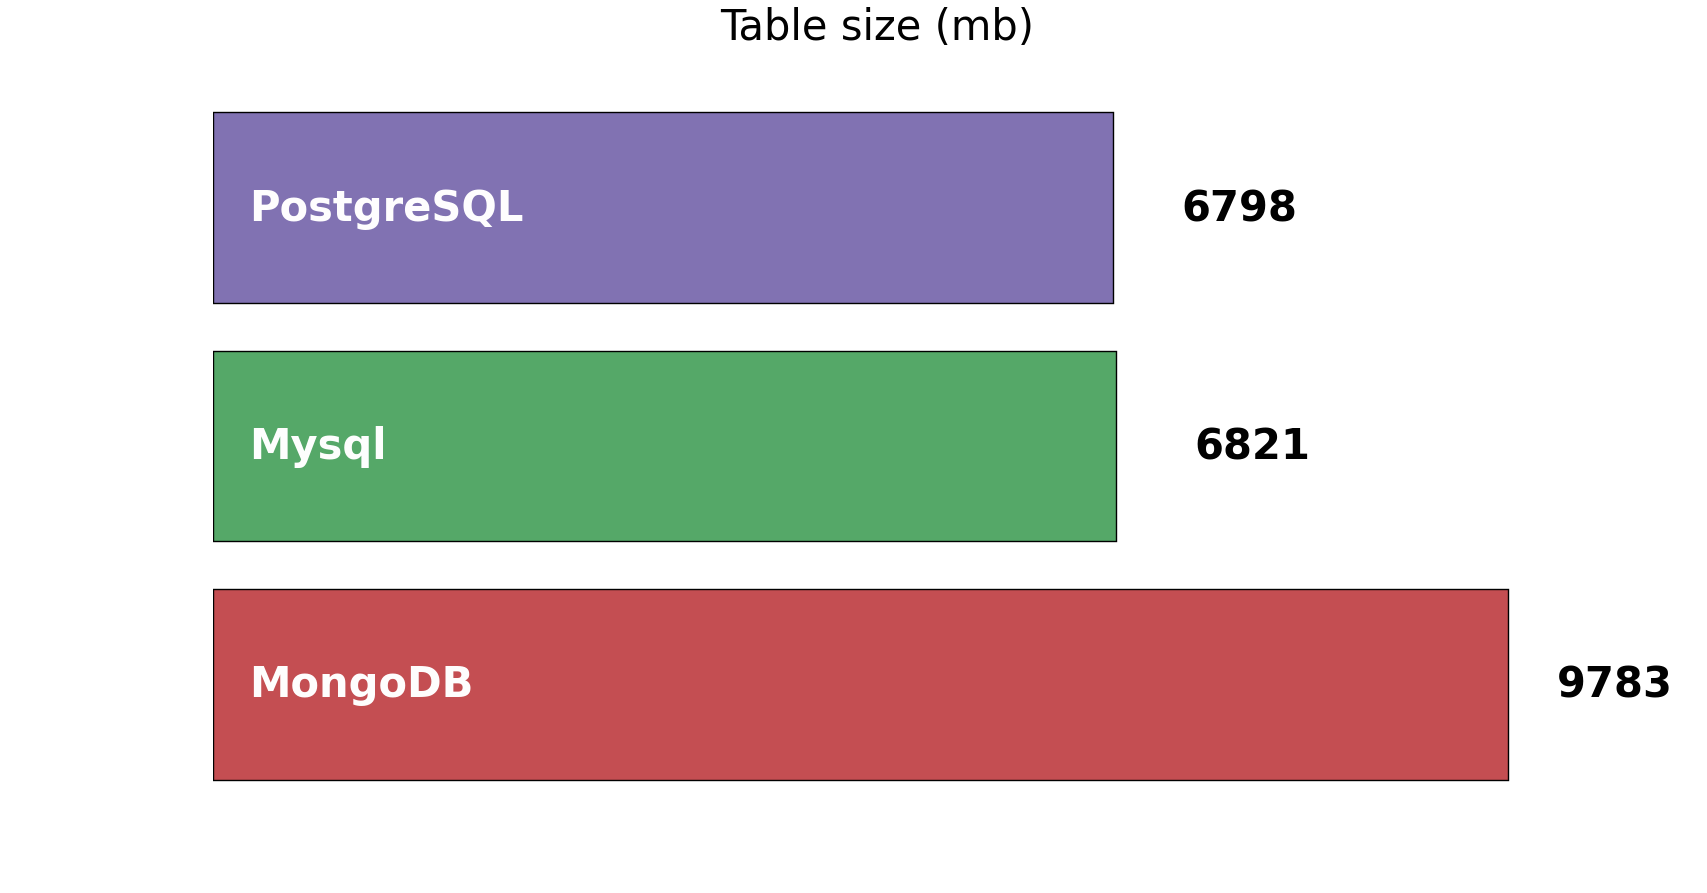
\includegraphics[width=0.95\textwidth,center]{benchmarks/table_size.png}
    %\end{figure}
    %\end{center}
%\end{frame}

%\begin{frame}
    %\frametitle{}
    %\begin{center}
    %\vspace{-10pt}
    %\textbf{Размер индексов}
    %\begin{figure}
        %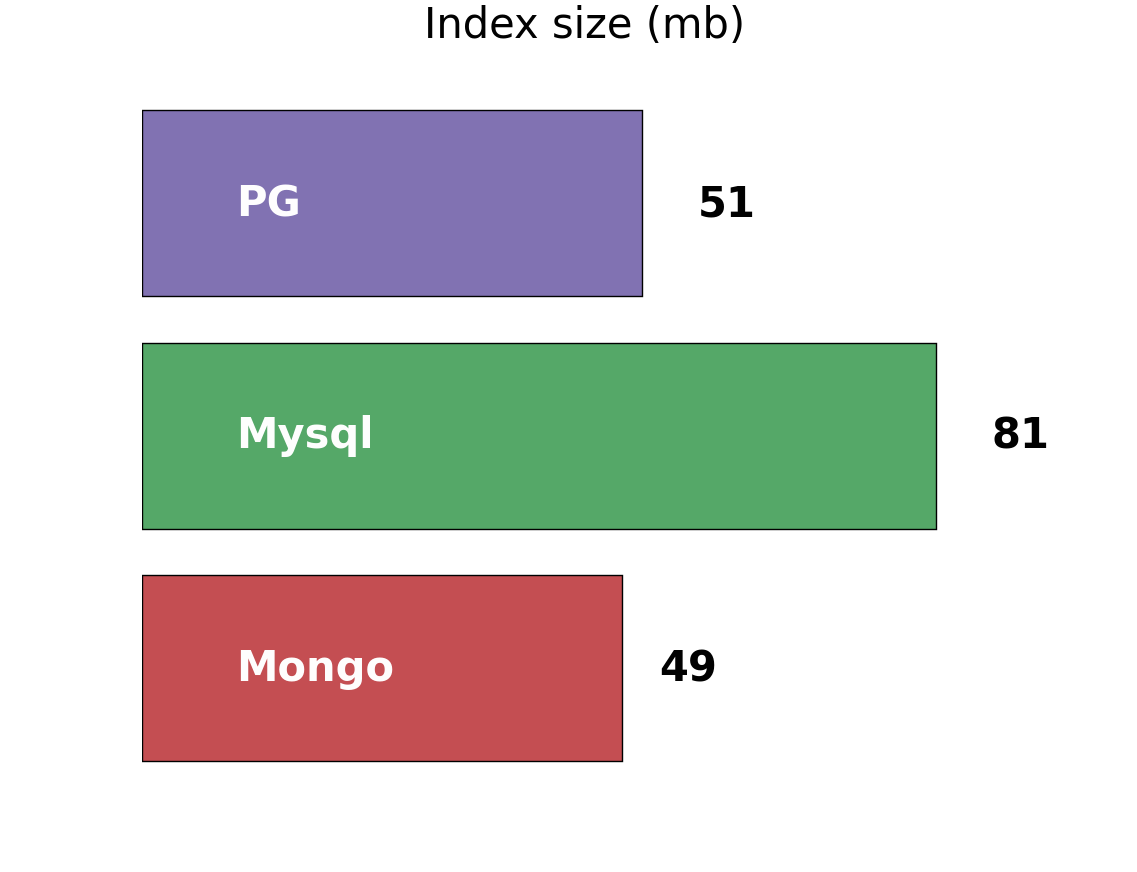
\includegraphics[width=0.7\textwidth,center]{benchmarks/index_size.png}
    %\end{figure}
    %\end{center}
%\end{frame}

%\begin{frame}
    %\frametitle{}
    %\begin{center}
    %\vspace{-10pt}
    %\textbf{Выборка документов с большим количеством ключей}
    %\end{center}
%\end{frame}
%\note{
    %сериализация в ширину
%}

%\begin{frame}
    %\frametitle{}
    %\begin{center}
    %\vspace{-10pt}
    %\textbf{Выборка документов с большой вложенностью}
    %\end{center}
%\end{frame}
%\note{
    %сериализация в глубину
%}

%\begin{frame}
    %\frametitle{}
    %\begin{center}
    %\vspace{-10pt}
    %\textbf{Выборка среза по документам}
    %\end{center}
%\end{frame}
%\note{
    %множественный detoast
%}

%\begin{frame}
    %\frametitle{}
    %\begin{center}
    %\vspace{-10pt}
    %\textbf{Выборка документов без кэша}
    %\end{center}
%\end{frame}
%\note{
    %моделирование ситуации, когда данные не влезают в память
    %и идет активная работа с диском
%}

%\begin{frame}
    %\frametitle{}
    %\begin{center}
    %\vspace{-10pt}
    %\textbf{SET STORAGE EXTERNAL}
    %\end{center}
%\end{frame}
%\note{
    %хранение jsonb в распакованном формате
%}

\begin{frame}
    \frametitle{}
    \begin{center}
        \textbf{Вставка документов}
        \begin{itemize}[label={}]
            \item "Простой документ"
            \item default write concern
        \end{itemize}
    \end{center}
\end{frame}

\begin{frame}
    \frametitle{}
    \begin{center}
    %\vspace{-10pt}
    \begin{figure}
        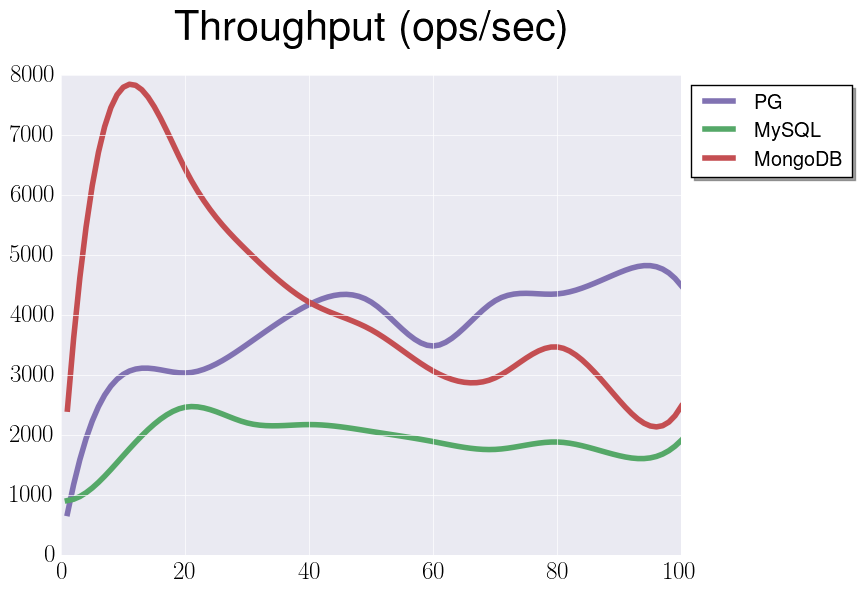
\includegraphics[width=0.75\textwidth,center]{benchmarks/insert_throughput.png}
    \end{figure}
    \end{center}
\end{frame}

\begin{frame}
    \frametitle{}
    \begin{center}
        \textbf{Вставка документов}
        \begin{itemize}[label={}]
            \item "Простой документ"
            \item journaled
        \end{itemize}
    \end{center}
\end{frame}

\begin{frame}
    \frametitle{}
    \begin{center}
    %\vspace{-10pt}
    \begin{figure}
        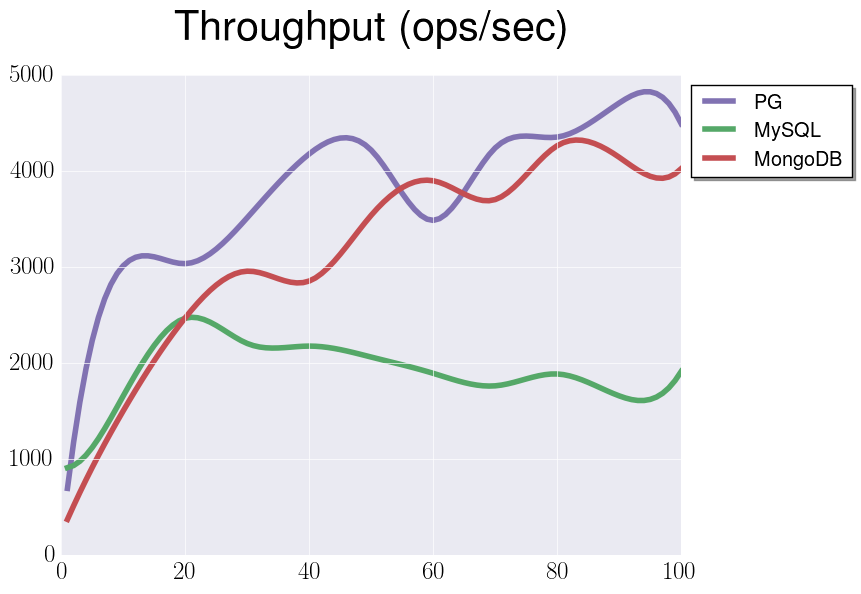
\includegraphics[width=0.75\textwidth,center]{benchmarks/insert_throughput_journaled.png}
    \end{figure}
    \end{center}
\end{frame}

\begin{frame}
    \frametitle{}
    \begin{center}
    %\vspace{-10pt}
    \begin{figure}
        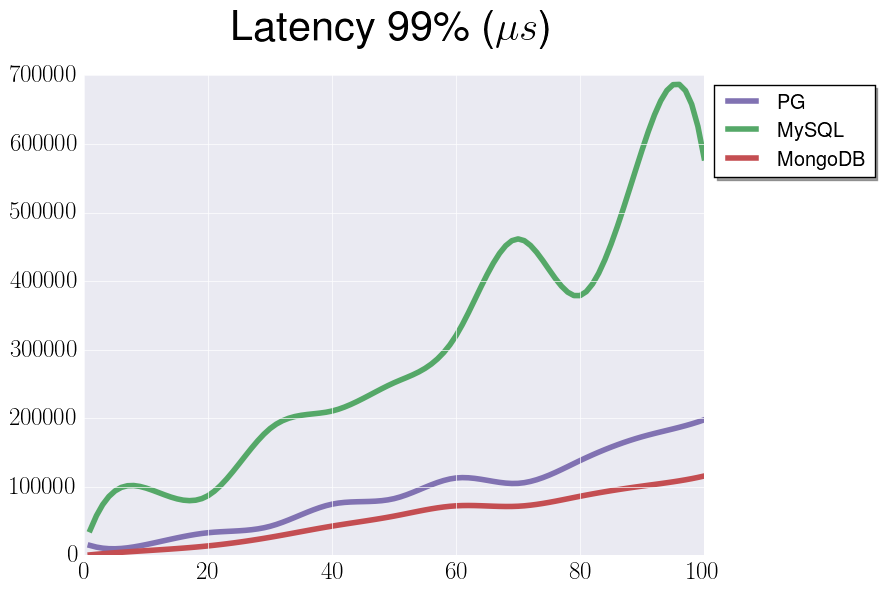
\includegraphics[width=0.75\textwidth,center]{benchmarks/insert_latency_99.png}
    \end{figure}
    \end{center}
\end{frame}

\begin{frame}
    \frametitle{}
    \begin{center}
        \textbf{Выборка 50\%, обновление 50\%}
        \begin{itemize}[label={}]
            \item "Простой документ"
            \item обновление одного поля
            \item transaction\_sync
        \end{itemize}
    \end{center}
\end{frame}

\begin{frame}
    \frametitle{}
    \begin{center}
    %\vspace{-10pt}
    \begin{figure}
        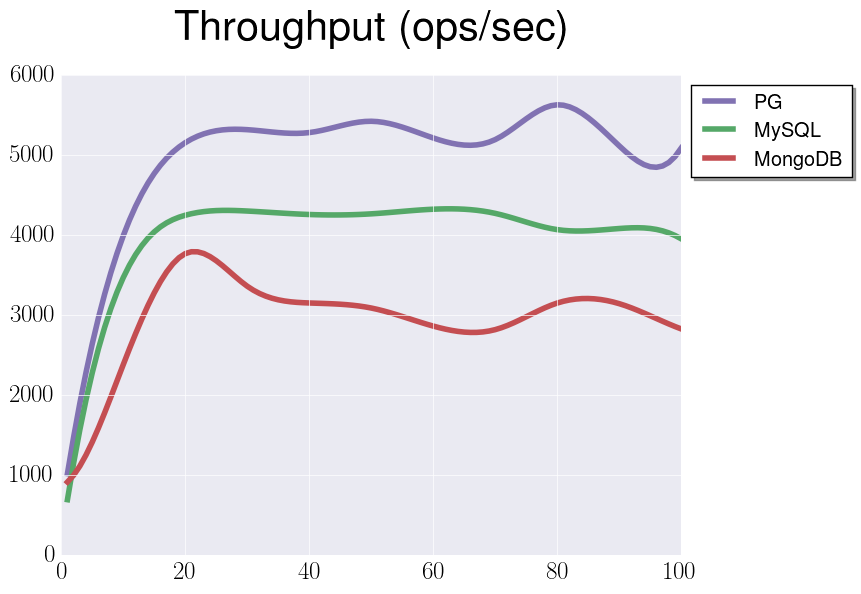
\includegraphics[width=0.75\textwidth,center]{benchmarks/update_btree_transaction_sync_throughput.png}
    \end{figure}
    \end{center}
\end{frame}

\begin{frame}
    \frametitle{}
    \begin{center}
    %\vspace{-10pt}
    \begin{figure}
        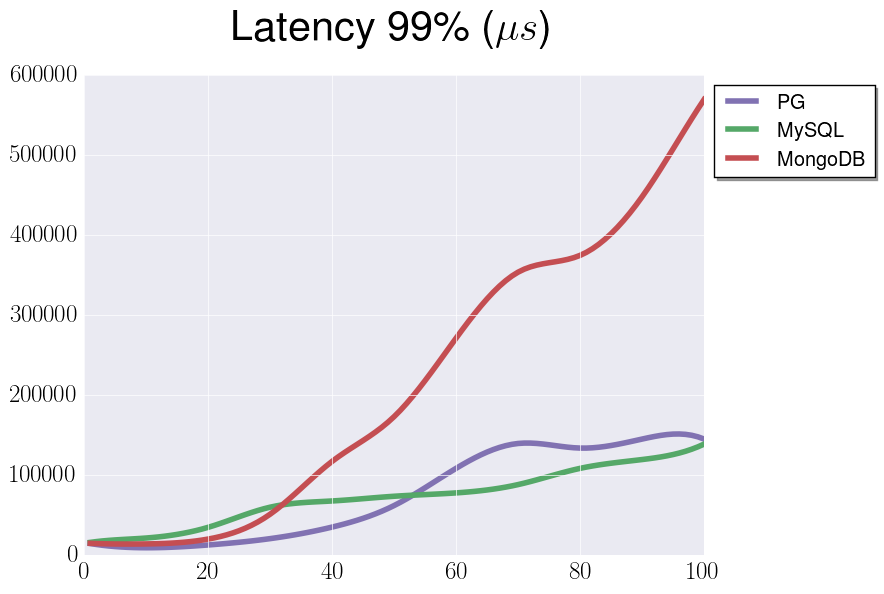
\includegraphics[width=0.75\textwidth,center]{benchmarks/update_btree_transaction_sync_latency.png}
    \end{figure}
    \end{center}
\end{frame}

\begin{frame}
    \frametitle{}
    \begin{center}
        \textbf{Выборка 50\%, обновление 50\%}
        \begin{itemize}[label={}]
            \item "Простой документ"
            \item обновление одного поля
            \item journaled
        \end{itemize}
    \end{center}
\end{frame}

\begin{frame}
    \frametitle{}
    \begin{center}
    %\vspace{-10pt}
    \begin{figure}
        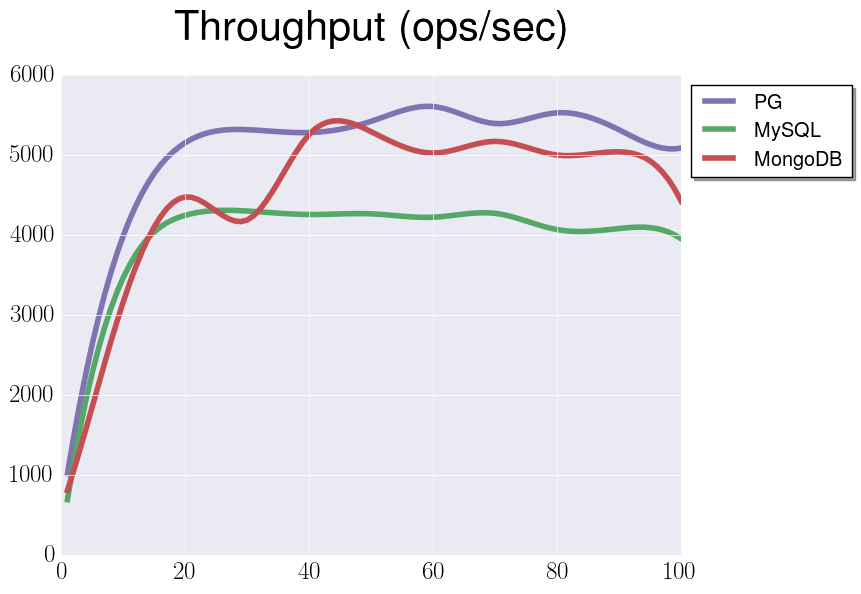
\includegraphics[width=0.75\textwidth,center]{benchmarks/update_btree_journaled_throughput.png}
    \end{figure}
    \end{center}
\end{frame}

\begin{frame}
    \frametitle{}
    \begin{center}
        \textbf{Выборка 50\%, обновление 50\%}
        \begin{itemize}[label={}]
            \item "Большой документ"
            \item обновление одного поля
        \end{itemize}
    \end{center}
\end{frame}

\begin{frame}
    \frametitle{}
    \begin{center}
    %\vspace{-10pt}
    \begin{figure}
        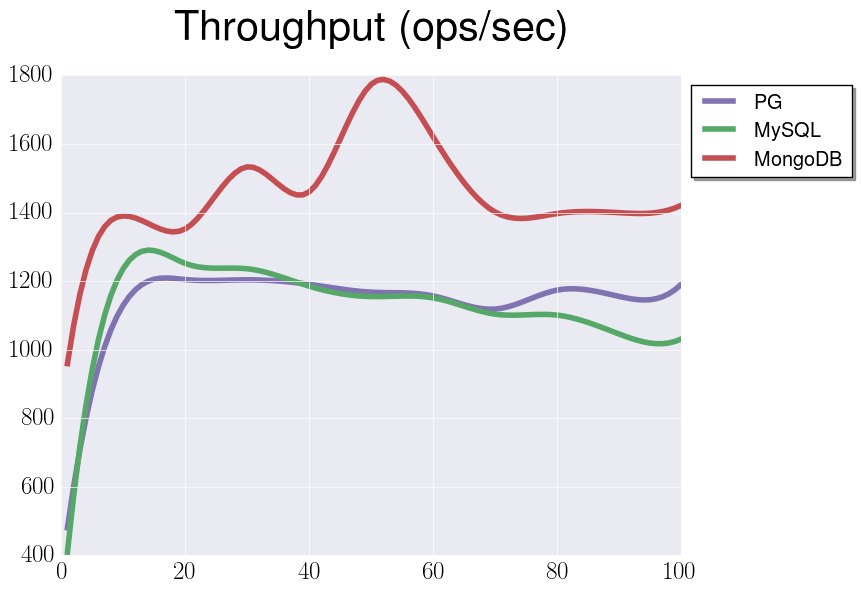
\includegraphics[width=0.75\textwidth,center]{benchmarks/update_btree_large_throughput.png}
    \end{figure}
    \end{center}
\end{frame}

\begin{frame}
    \frametitle{}
    \begin{center}
    %\vspace{-10pt}
    \begin{figure}
        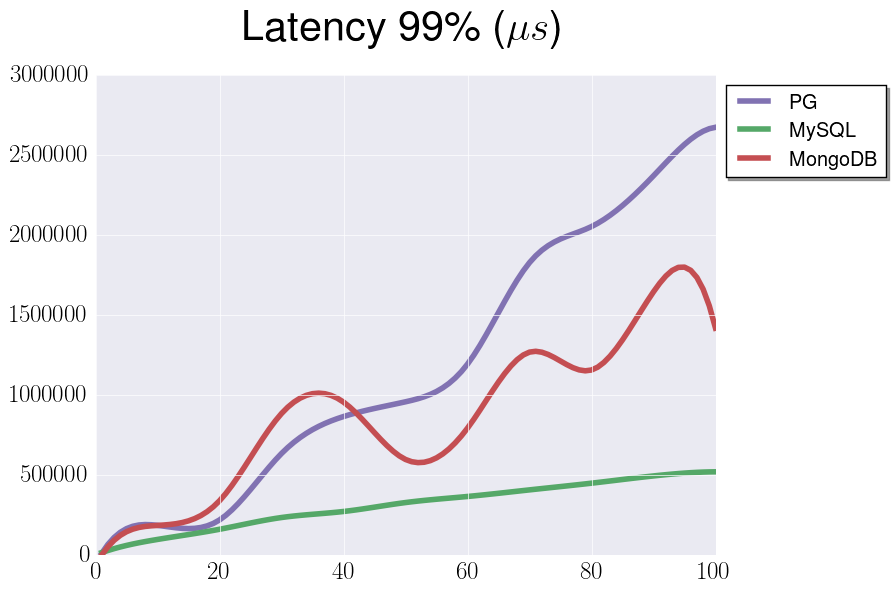
\includegraphics[width=0.75\textwidth,center]{benchmarks/update_btree_large_latency.png}
    \end{figure}
    \end{center}
\end{frame}

%\begin{frame}
    %\frametitle{}
    %\begin{center}
    %\vspace{-10pt}
    %\textbf{Вставка записей}
    %\end{center}
%\end{frame}

%\begin{frame}
    %\frametitle{}
    %\begin{center}
    %\vspace{-10pt}
    %\textbf{Вставка и обновление}
    %\end{center}
%\end{frame}

%\begin{frame}
    %\frametitle{}
    %\begin{center}
    %\vspace{-10pt}
    %\textbf{Чтение последних}
    %\end{center}
%\end{frame}

%\begin{frame}
    %\frametitle{}
    %\begin{center}
    %\vspace{-10pt}
    %\textbf{Чтение, изменение, запись}
    %\end{center}
%\end{frame}

\begin{frame}[fragile]
    \frametitle{}
    \vspace{10pt}
    \begin{itemize}[leftmargin=*, label={\MVRightarrow}]
        \item <+-> Документов в RDBMS можно не бояться
        \item <+-> Приведенные бенчмарки - "подсказки"
        \item <+-> Необходимы свои тесты для нагрузки
    \end{itemize}
\end{frame}
\note{
    чтение, поиск и вставка - "правильный вид нагрузки" для реляционной базы данных по мнению финна Markus Winand
}

\usebackgroundtemplate{
\includegraphics[width=\paperwidth]{title_background.png}}%
\fontsize{17pt}{18}\selectfont
\begin{frame}
  \vspace*{2.5cm}
  \begin{columns}[T,onlytextwidth]
  \column{0.3\textwidth}
  \column{0.7\textwidth}
  \begin{minipage}[b][\paperheight]{\textwidth}

      \raggedright%
      \linespread{1.0}%
      \usebeamerfont{title}%
      \usebeamercolor[fg]{title}%
      \if@noSmallCapitals%
        Вопросы?
      \else%
        \scshape\MakeLowercase{Вопросы?}%
      \fi%
      \vspace*{0.3em}

      \usebeamerfont{subtitle}%
      \fontsize{13pt}{14}\selectfont
      \usebeamercolor[fg]{subtitle}%
        \begin{itemize}[label={}]
            \item {\github\ github.com/erthalion}
            \item {\twitter\ @erthalion}
            \item \email\ 9erthalion6 at gmail dot com
        \end{itemize}
      \vspace*{2.5em}%

    \begin{columns}[T,onlytextwidth]
    \column{0.32\textwidth}
      \usebeamerfont{author}%
      \usebeamercolor[fg]{author}%
      \insertauthor%
      \vspace*{0.5em}%
    \column{0.32\textwidth}
      \usebeamerfont{author}%
      \usebeamercolor[fg]{author}%
      Senior Software Engineer
      \vspace*{0.5em}%
    \column{0.32\textwidth}
      \usebeamerfont{author}%
      \usebeamercolor[fg]{author}%
      Zalando
      \vspace*{0.5em}%
    \end{columns}

    \vfill
    \vspace*{2em}
  \end{minipage}
  \end{columns}

\end{frame}

\end{document}
